\documentclass[xcolor=table, aspectratio=169,ignorenonframetext]{beamer}

%\usepackage{arev}
\usepackage{amsmath,amssymb,amscd}
\usepackage{dsfont}
\usepackage{mathrsfs}
\usepackage{yfonts}
\usepackage{bm}
\usepackage{graphicx}
\usepackage{tabularx}
\usepackage{animate}
\usepackage{listings}
%\usepackage{ifthen}
\usepackage{pifont}

\usepackage{xeCJK}
\usepackage{fontspec}
\newfontfamily\cjkfont{WenQuanYi Zen Hei}
\setCJKmainfont{WenQuanYi Zen Hei}
%\newfontfamily\cjkfont{PingFang SC}
%\setCJKmainfont{PingFang SC}
\newcolumntype{x}{>{\centering\arraybackslash}X}
\renewcommand{\arraystretch}{1.5}
\DeclareMathOperator{\img}{img}
\DeclareMathOperator{\hhom}{Hom}
\newcommand{\uone}{\text U(1)}
\DeclareMathOperator{\id}{id}
\usepackage{tikz}
	\usetikzlibrary{calc}
	\usetikzlibrary{arrows,shapes, positioning, matrix}
	\usetikzlibrary{decorations.markings}
	\tikzstyle arrowstyle=[scale=1]
  \tikzstyle string=[thick,postaction={decorate,decoration={markings,
      mark=at position .55 with {\arrow[arrowstyle]{stealth}}}}]

\usepackage{tikz-cd}
\usepackage{pgffor}
\newcommand{\cohosub}[1]{\scalebox{0.72}{\textswab{#1}}}
\newcommand{\cohosubsub}[1]{\scalebox{0.6}{\textswab{#1}}}
\newcommand{\coho}[1]{\textswab{#1}}


\mode<presentation>
{
  %\usetheme{Warsaw}
  % or ...
  %\useoutertheme{rectangle}
  \setbeamertemplate{frametitle}[default][center]
  \defbeamertemplate{itemize item}{flat}{\begin{pgfpicture}{-1ex}{0ex}{1ex}{2ex}
      \pgfpathcircle{\pgfpoint{0pt}{.6ex}}{0.6ex}
      \pgfusepath{fill}
    \end{pgfpicture}%
  }
  \defbeamertemplate{itemize subitem}{flat}{\footnotesize\raise0.5pt\hbox{\textbullet}}
  \defbeamertemplate{itemize subsubitem}{flat}{\footnotesize\raise0.5pt\hbox{\textbullet}}

  %\useinnertheme{circles}
  \setbeamertemplate{items}[flat]
  \setbeamertemplate{sections/subsections in toc}[circle]
  \setbeamertemplate{blocks}[rounded]
  \setbeamertemplate{title page}[default][colsep=-4bp,rounded=true]
  \setbeamertemplate{part page}[default][colsep=-4bp,rounded=true]
  \setbeamercovered{transparent}
  %\usecolortheme{spruce}
  %\definecolor{THU}{RGB}{116,61,130}
  \definecolor{mbg}{RGB}{0,0,160}
  \setbeamercolor*{palette primary}{fg=white,bg=mbg}
  \setbeamercolor*{titlelike}{parent=palette primary}
  \setbeamercolor*{structure}{fg=mbg}
  \setbeamercolor{frametitle}{fg=white,bg=mbg}
  % or whatever (possibly just delete it)
  \setbeamercolor{block title}{bg=mbg,fg=white}
  \setbeamercolor{block body}{bg=mbg!15}


  \addtobeamertemplate{navigation symbols}{}{ \hspace{1em}%
    \usebeamerfont{footline}%
    \insertframenumber / \inserttotalframenumber }
}


%\usepackage[english]{babel}
% or whatever

%\usepackage[latin1]{inputenc}
% or whatever

%\usepackage{times}
%\usepackage[T1]{fontenc}
% Or whatever. Note that the encoding and the font should match. If T1
% does not look nice, try deleting the line with the fontenc.

\title % (optional, use only with long paper titles)
{Computing the classification of symmetry-protected topological phases with homological algebra}
\author[Y Qi] % (optional, use only with lots of authors)
{Yang~Qi}
% - Give the names in the same order as the appear in the paper.
% - Use the \inst{?} command only if the authors have different
%   affiliation.

\institute[Fudan] % (optional, but mostly needed)
{
Department of Physics, Fudan University.
}
% - Use the \inst command only if there are several affiliations.
% - Keep it simple, no one is interested in your street address.

%\date{2016 Annual Meeting of Fudan CFTPP} % (optional, should be abbreviation of conference name)
%{Fudan University, Oct 13 2015}
\date{Oct. 17th, 2020}
% - Either use conference name or its abbreviation.
% - Not really informative to the audience, more for people (including
%   yourself) who are reading the slides online

%\subject{Theoretical Physics}
% This is only inserted into the PDF information catalog. Can be left
% out.



% If you have a file called "university-logo-filename.xxx", where xxx
% is a graphic format that can be processed by latex or pdflatex,
% resp., then you can add a logo as follows:

\pgfdeclareimage[height=1cm]{university-logo}{../resources/fudan}
\logo{\pgfuseimage{university-logo}}



% Delete this, if you do not want the table of contents to pop up at
% the beginning of each subsection:
\AtBeginSection[]
{
  \begin{frame}<beamer>{Outline}
			\tableofcontents[currentsection,currentsubsection]
  \end{frame}
}
%\AtBeginSubsection[]
%{
 % \begin{frame}<beamer>{Outline}
  %  \tableofcontents[currentsection,currentsubsection]
  %\end{frame}
%}


\begin{document}

\begin{frame}
  \titlepage
\end{frame}

\begin{frame}{References}
\begin{itemize}
\item[Beihang Univ.] 李伟, 李涵
\item Chen Fang: Institute of Physics, Beijing.
\item Yunqing Ouyang: Fudan University.
\item Qing-Rui Wang: Yale University.
\item Zheng-Cheng Gu: Chinese University of Hong Kong.
\begin{center}
	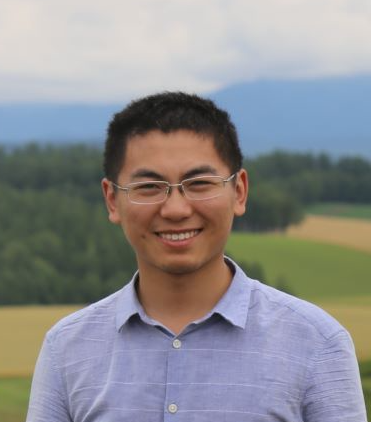
\includegraphics[height=2cm]{../people/zhidasong}
	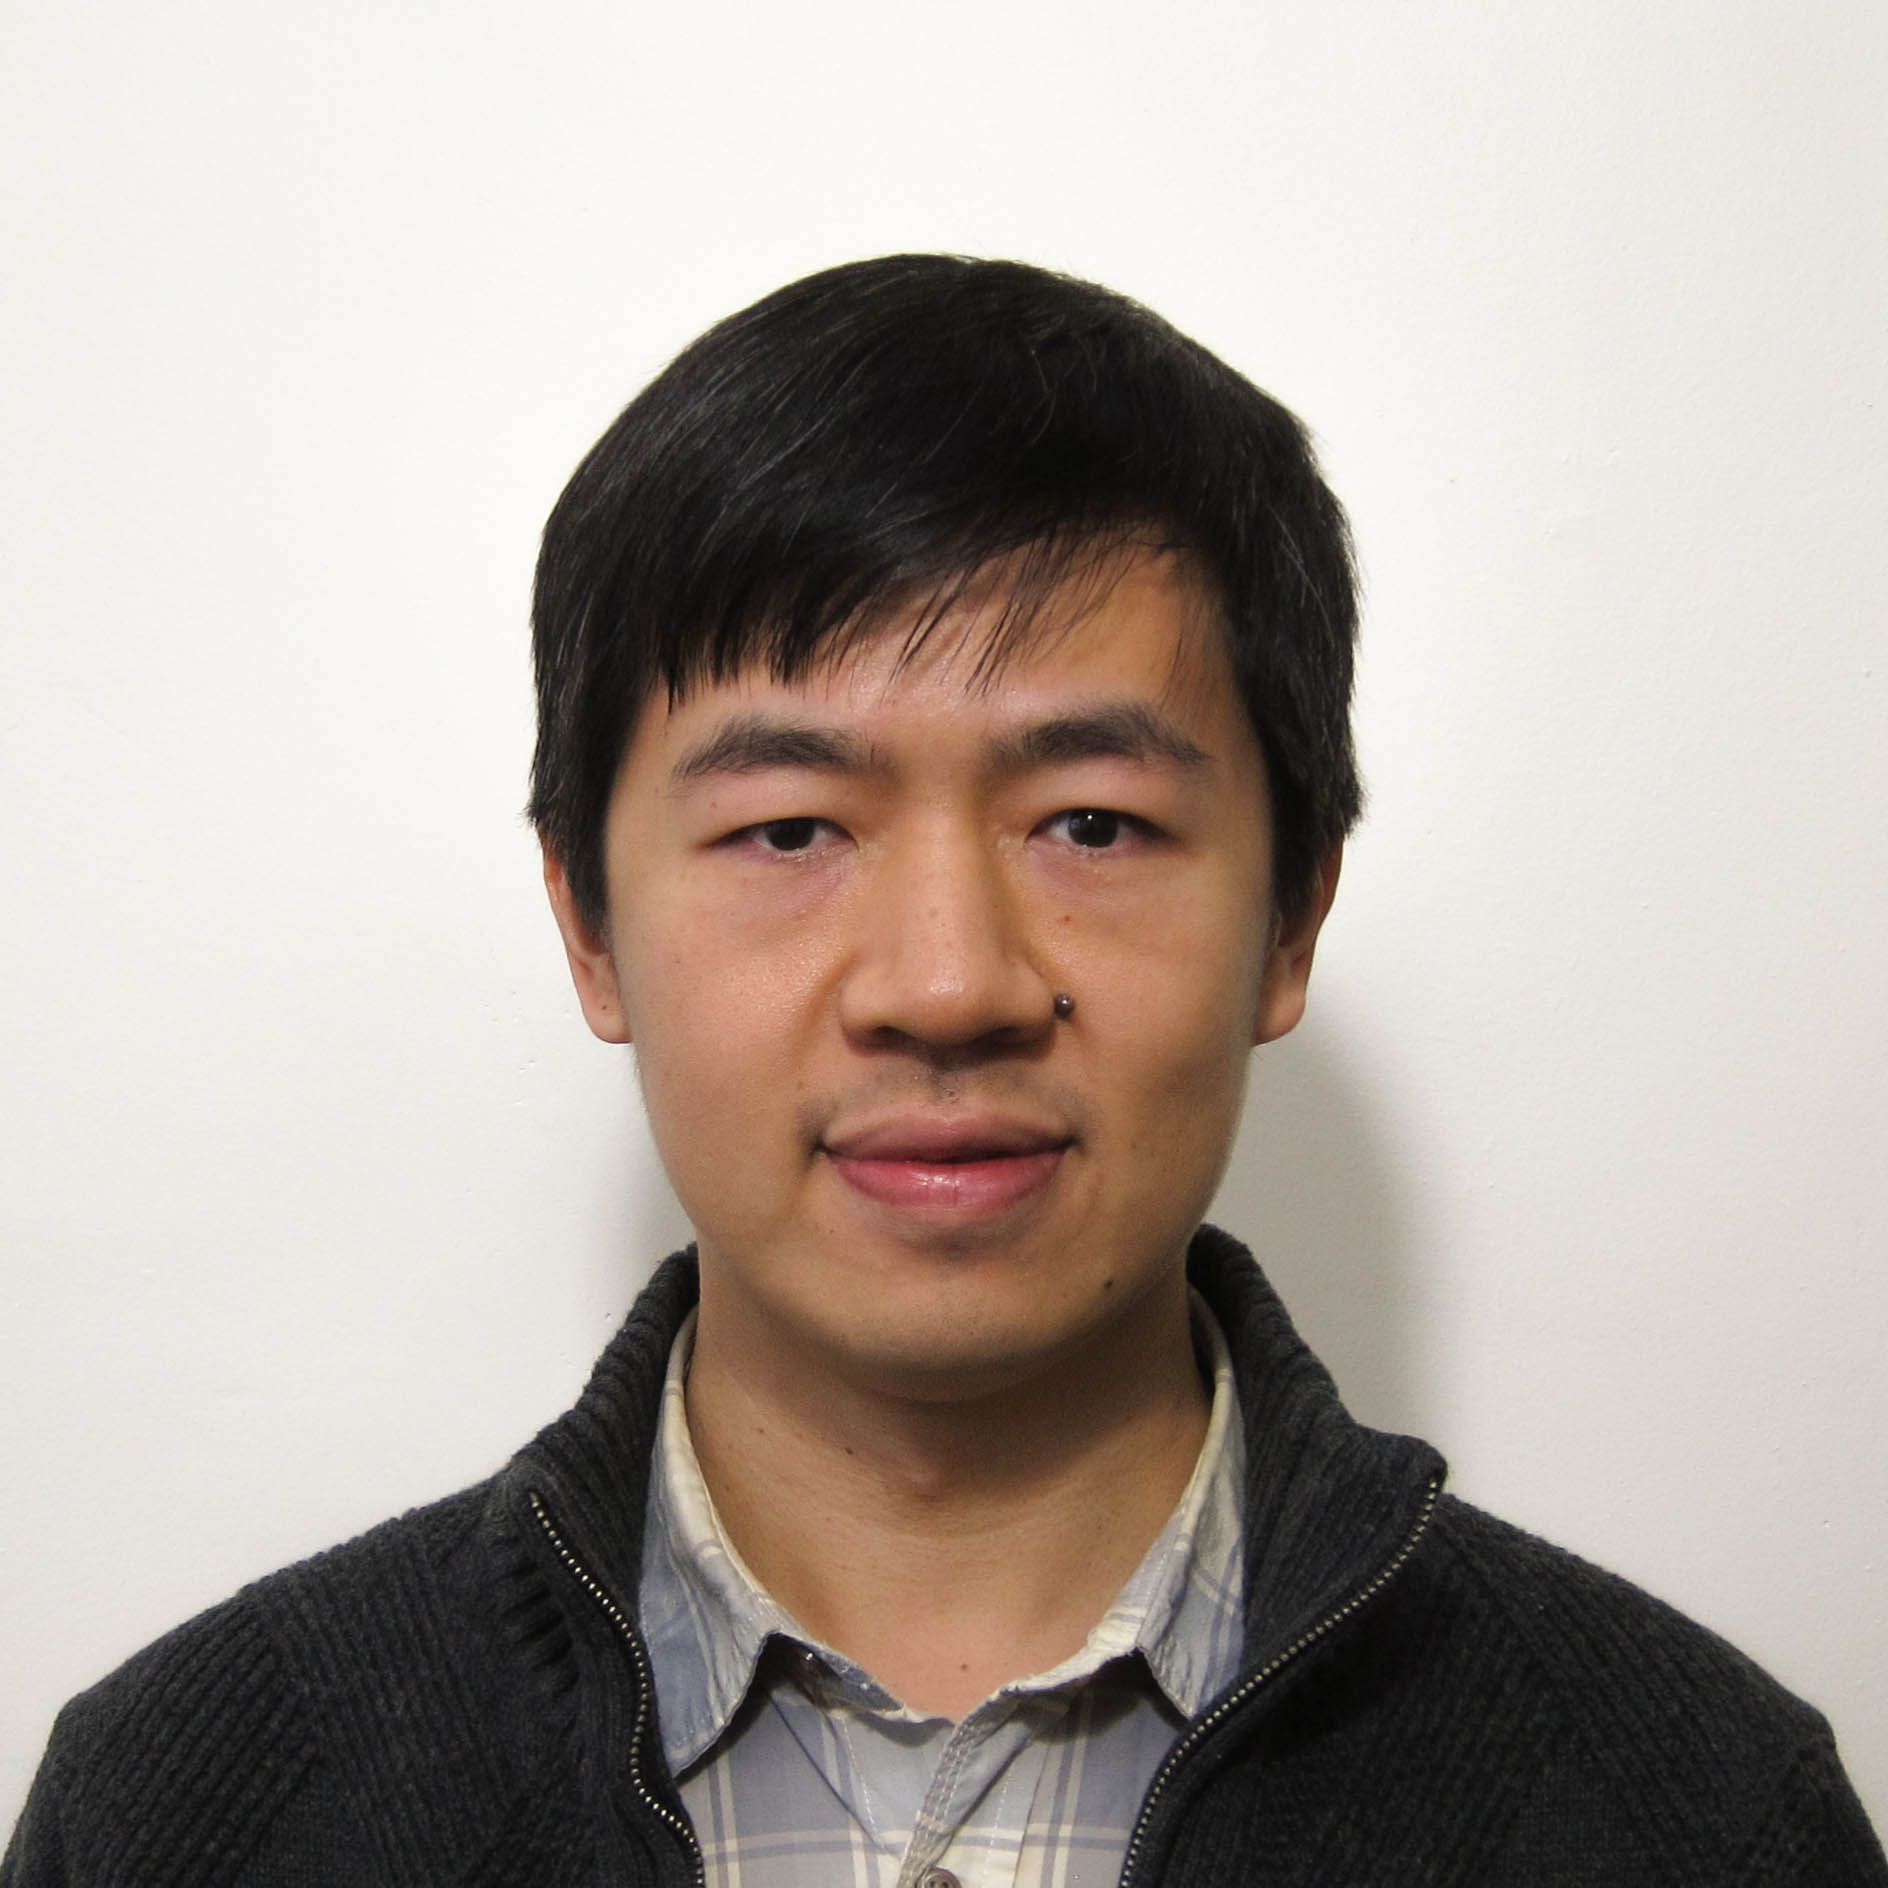
\includegraphics[height=2cm]{../people/chenfang}
        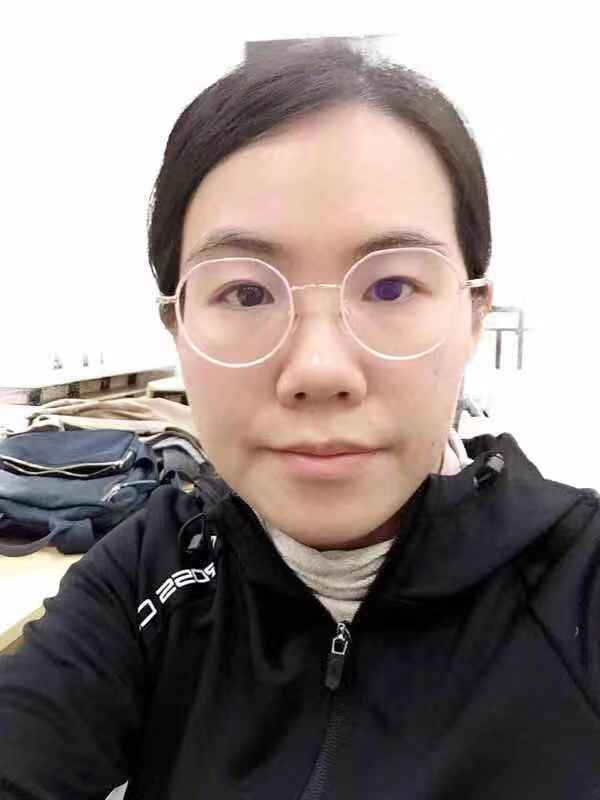
\includegraphics[height=2cm]{../people/yunqing}
        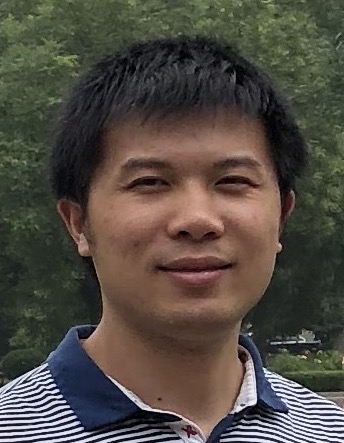
\includegraphics[height=2cm]{../people/qingrui}
        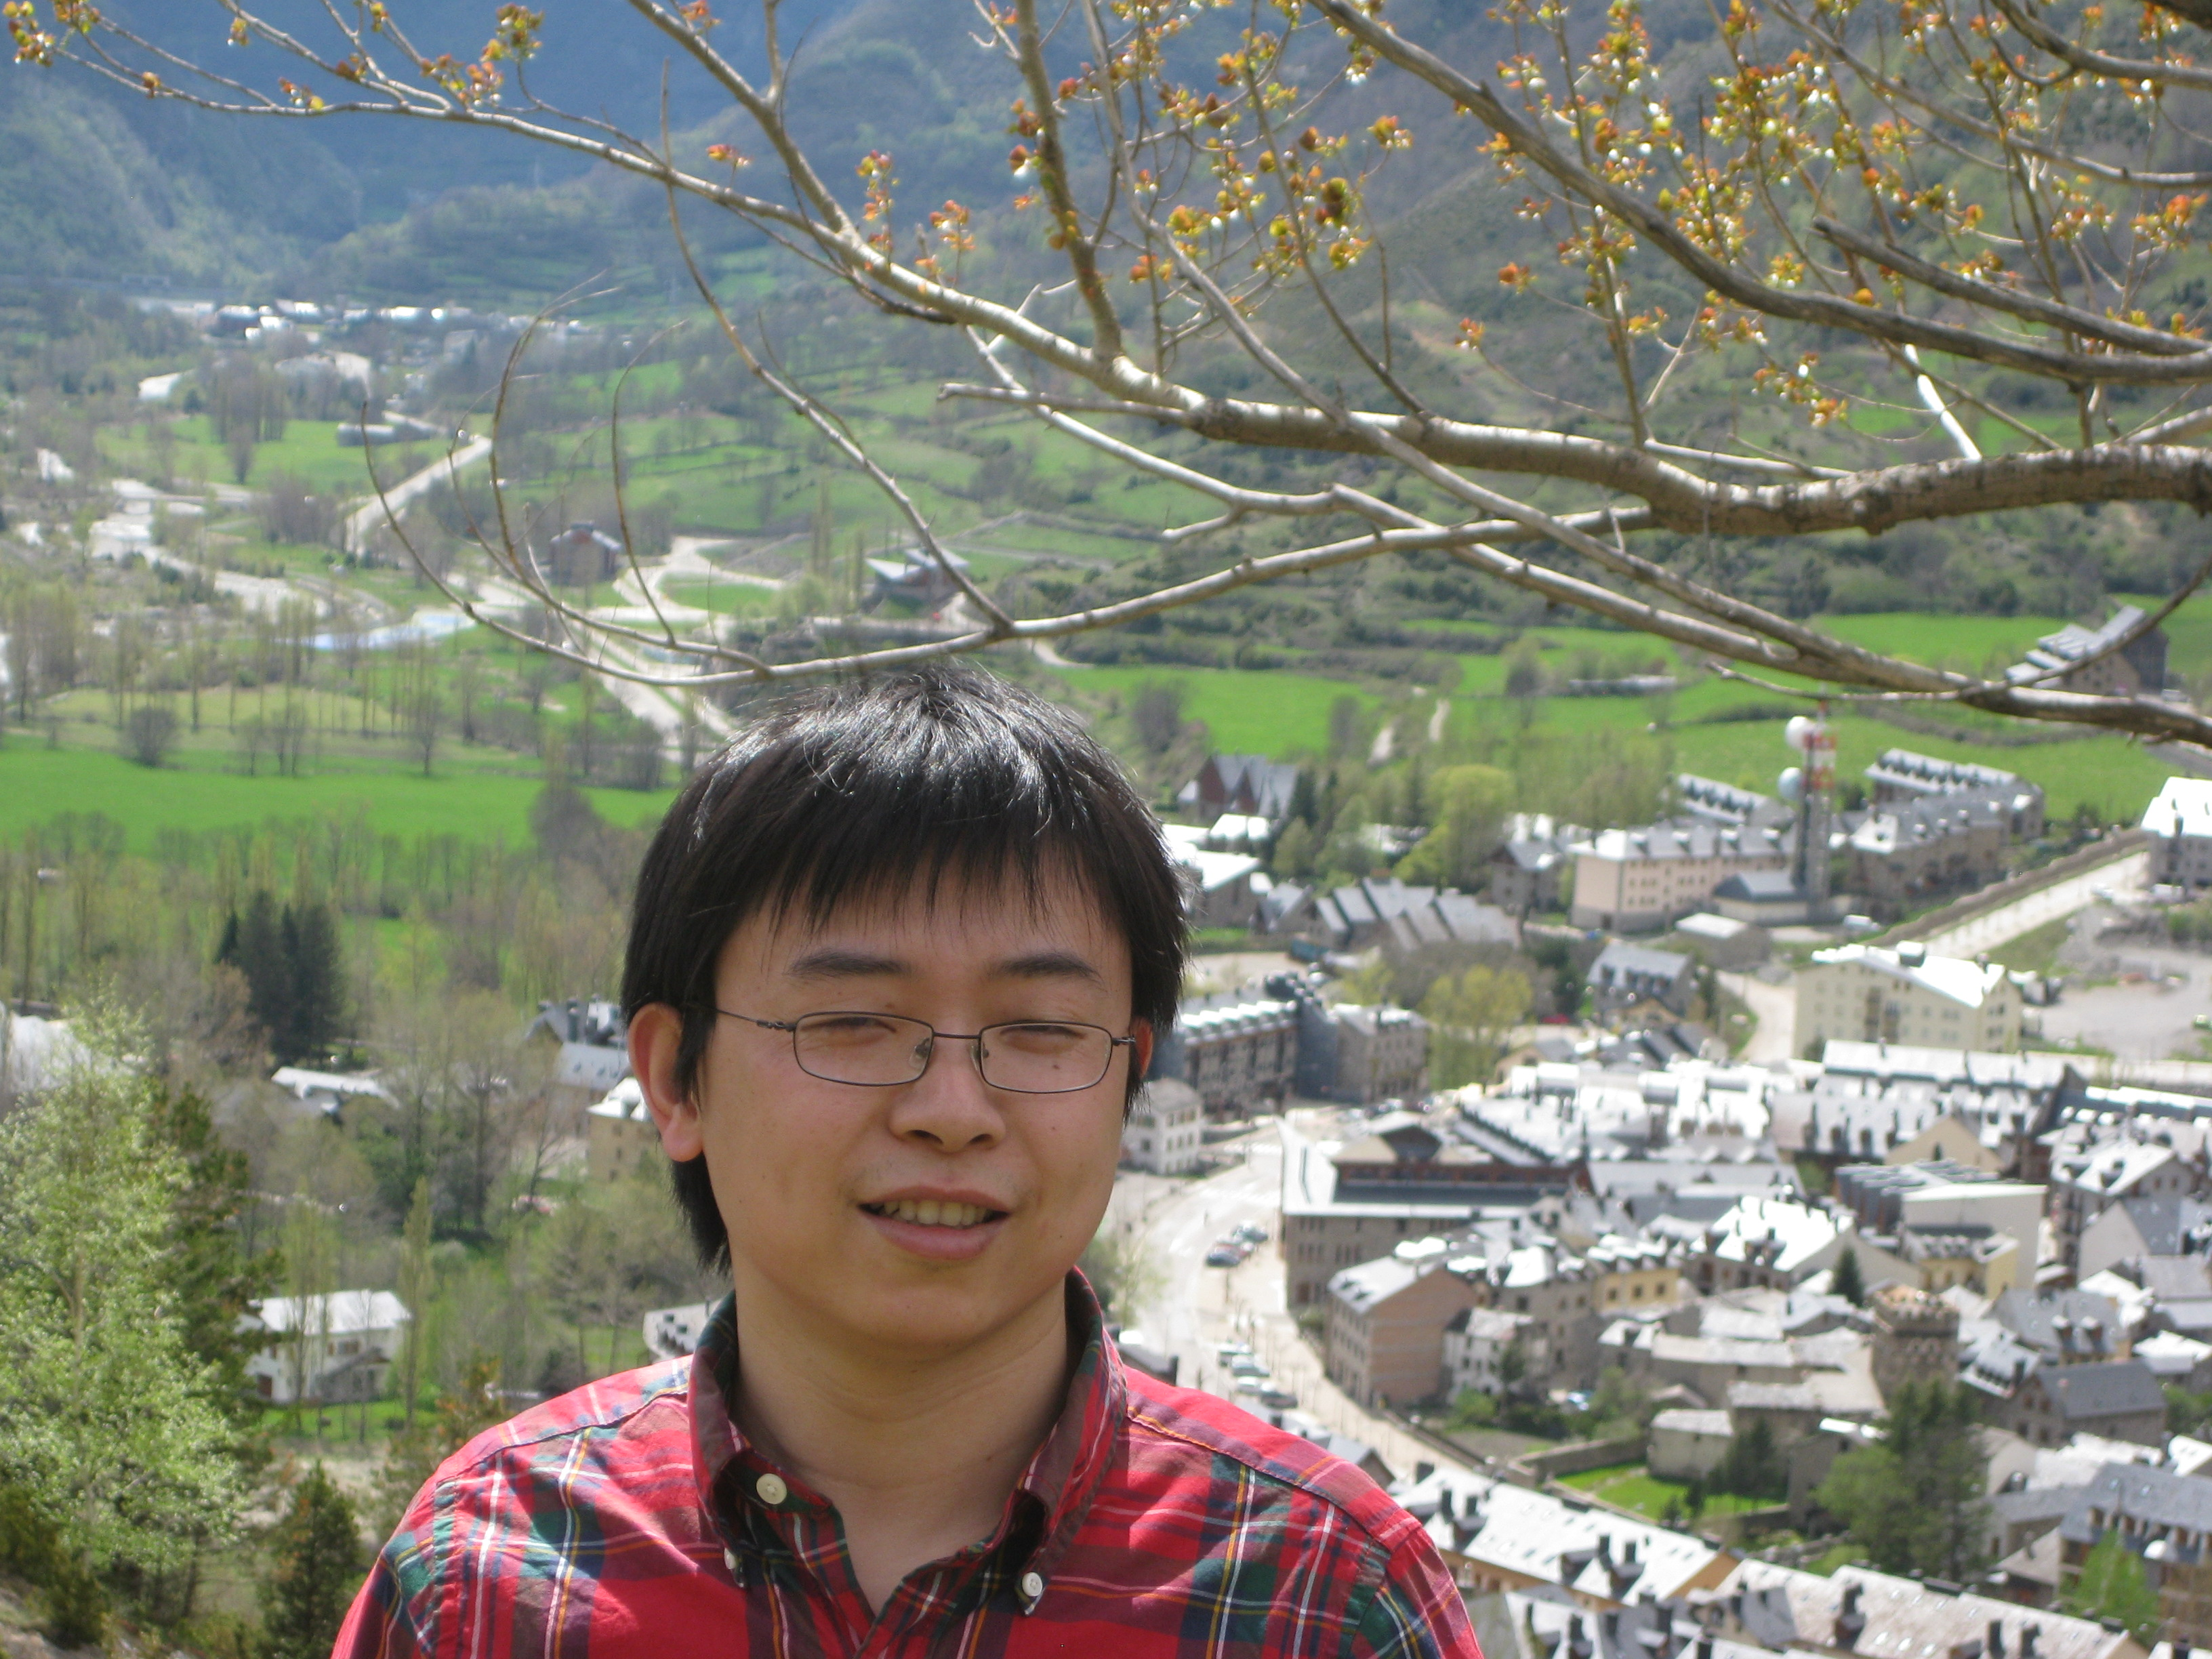
\includegraphics[height=2cm]{../people/zhengcheng}
\end{center}
\item Zhida Song, Chen Fang and Yang Qi, Nature Communications \textbf{11}, 4197 (2020).
\item Yunqing Ouyang, Qing-Rui Wang, Zheng-Cheng Gu and Yang Qi, arXiv:2005.06572.
\end{itemize}
\end{frame}

\begin{frame}{Outline}
	%\begin{columns}
	%\column{.7\textwidth}
		\tableofcontents
  %\end{columns}
  % You might wish to add the option [pausesections]
\end{frame}

\section{Introduction to SPT states}

\end{document}

%%% Local Variables: 
%%% coding: utf-8
%%% mode: latex
%%% TeX-engine: xetex
%%% End: 